\documentclass[12pt]{article}

\usepackage{amsmath}
\usepackage{amsfonts}
\usepackage{amssymb}
\usepackage{xcolor}
\usepackage[siunitx, RPvoltages]{circuitikz}
\usepackage{empheq}
\usepackage{hyperref}
\usepackage{pgfplots}
\usepackage{fullpage}
\usepackage{caption}
\usepackage{subcaption}
\usepackage{upgreek}


\pgfplotsset{width=7cm, compat=1.16}

\counterwithin{figure}{section}
\numberwithin{equation}{section}

\newcommand*\widefbox[1]{\fbox{\hspace{2em}#1\hspace{2em}}}

\hypersetup{
	colorlinks,
	citecolor=black,
	filecolor=black,
	linkcolor=blue,
	urlcolor=cyan,
}

\title{\textbf{Time Domain Analysis}}
\author{Jay Khandkar}
\date{January 18, 2021}

\begin{document}

\maketitle
\newpage
\tableofcontents
\newpage
\begin{flushleft}
\color{blue}
\section{Current And Voltage Conventions}
\color{black}

The conventions we shall follow simply state that when 
current ``flows into" the positive terminal of the capacitor/inductor, as indicated by the polarity of $v$
in Fig.\ref{fig:conventions}, it is taken as positive. We may then write the current-voltage relations:

\begin{empheq}[box=\widefbox]{align*}
i &= C\frac{dv}{dt}\\
v &= L\frac{di}{dt}
\end{empheq}

\begin{figure}[h!]
\centering
\fbox{
\begin{circuitikz}[american]
	
	\draw (0,0) to[short, i=$i$] (1,0) to[C, l=$C$, v_=$v$, o-o, voltage shift=2.5] (2,0) 
	to[short] (3,0);
	\draw (0,-2) to[short, i=$i$] (1,-2) to[cute inductor, l=$L$, v^=$v$, o-o, voltage shift=5.0] (2,-2) 		to[short] (3,-2);
	
\end{circuitikz}
}
\caption{The voltage conventions}
\label{fig:conventions}	
\end{figure}

\color{blue}
\section{First Order Circuits: RL and RC}
\color{black}
A first order circuit is one that is governed by a first order differential equation. Often, it is
incorrectly stated that a first order circuit is one that contains only one energy storage element
(capacitor/inductor). This is wrong, as there are certain arrangements of $R-L$ and $R-C$ circuits
which can be simplified to obtain a first order equation, as we shall see later. So, there being only
one energy storage element in a circuit is a \textit{sufficient} but not \textit{necessary} condition for
it to be first order.

\color{blue}
\subsection{The Natural Response}
\subsubsection{The Source-Free RL Circuit}
\color{black}
A \textbf{\textit{natural response}} is one that is free of any external voltage/current sources, 
which are also known as \textit{forcing functions}. It depends on the ``general nature" of the circuit (types of elements, sizes and interconnections). It is also known as the \textbf{\textit{transient response}}, as without any external sources, it must eventually die out. Consider the simple series RL
circuit shown in Fig.\ref{fig:src_free_RL}:
\newpage
\begin{figure}[!h]
\centering
\begin{circuitikz}[american]
	\draw (0,0) to [R=$R$, v>=$v_R$, voltage shift=2.5] (0,3) to [short, i=$i(t)$] (3,3)
			to [cute inductor, l=$L$, v=$v_L$] (3,0) to [short] (0,0); 
\end{circuitikz}
\caption{Simple R-L circuit for which $i(t)$ is to be determined}
\label{fig:src_free_RL}	
\end{figure}

Let the time varying current be designated $i(t)$, and the value of $i$ at $t=0$ be $I_0$. It may seem 
counter-intuitive to have a non-zero current initially in a circuit with no sources. In order 
for a current to be flowing, a source had to be present at some point of time, but we are only bothered with the response of the circuit after $t=0$, ie. after the source has been removed. Applying Kirchhoff's
voltage law, we have
\begin{equation*}
Ri + v_L = Ri + L\frac{di}{dt} = 0 
\end{equation*}
or
\begin{equation}
\label{equation:rl_natural}
\frac{di}{dt} + \frac{R}{L}i = 0
\end{equation}
We can separate variables and integrate easily, giving

\begin{equation}
\label{equation:rl_nat_resp}
\boxed{i(t) = I_0e^{-\frac{R}{L}t}}
\end{equation}

where we have incorporated the intitial codition $i(0)=I_0$. The general form of the natural response will 
be
\begin{equation}
\boxed{i(t) = Ke^{-\frac{R}{L}t}}
\end{equation}
where $K$ is a constant, and is nothing but the value of $i$ at $t=0$.

\paragraph{\color{blue}Accounting For The Energy}\mbox{} \\ \mbox{}\\
The power dissipated through the resistor at any time $t$

\begin{equation*}
p_R = i^{2}R = I_0^{2}Re^{-\frac{2Rt}{L}}
\end{equation*}

and the total energy turned into heat by the resistor till the response has died out

\begin{align*}
w_R &= \int_{0}^{\infty} p_R\,dt\\
    &= I_0^{2}R\int_{0}^{\infty} e^{-\frac{2Rt}{L}}\,dt\\
    &= I_0^{2}R\left (\frac{-L}{2R}\right)e^{-\frac{2Rt}{L}}\Biggr|_{0}^{\infty}\\
\Aboxed{w_R &= \frac{1}{2}LI_0^{2}}
\end{align*}
which is the total energy stored initially in the inductor, as expected.

\color{blue}
\subsubsection{Properties Of The Natural Response}
\color{black}

\begin{figure}[!h]
\centering
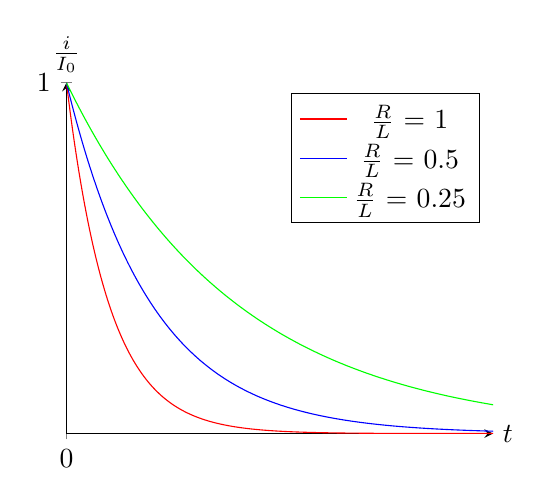
\begin{tikzpicture}
\begin{axis}[
	legend pos = north east,
    axis lines = left,
    ytick={1}, xtick={0},
    x label style = {at={(1,0)},anchor=west},
    y label style = {at={(0,1)},rotate=-90,anchor=south},
    xlabel = $t$,
    ylabel = {$\frac{i}{I_0}$},
]

\addplot [
    domain=0:10, 
    samples=100, 
    color=red, smooth
]
{exp(-x)};
\addlegendentry{$\frac{R}{L}$ = 1}
\addplot [
    domain=0:10, 
    samples=100, 
    color=blue, smooth
]
{exp(-0.5*x)};
\addlegendentry{$\frac{R}{L}$ = 0.5}
\addplot [
    domain=0:10, 
    samples=100, 
    color=green, smooth
]
{exp(-0.25*x)};
\addlegendentry{$\frac{R}{L}$ = 0.25}

\end{axis}
\end{tikzpicture}
\caption{Some possible plots for the natural response}
\label{fig:nat_resp}
\end{figure}

From the natural response of the series RL circuit given by Eq.\ref{equation:rl_nat_resp}, it is clear that
that the current decays exponentially to zero from an initial value of $I_0$. The graph of $\frac{i}{I_0}$
is plotted in figure \ref{fig:nat_resp} for three different values of $\frac{R}{L}$, as indicated in the legend.

Consider now the initial rate of decay, which is found by differentiating equation \ref{equation:rl_nat_resp}:

\begin{equation*}
\frac{d}{dt}\frac{i}{I_0}\Biggr|_{t=0} = -\frac{R}{L}e^{-Rt/L}\Biggr|_{t=0} = -\frac{R}{L}
\end{equation*}
Assuming that the decay continues at this rate, the time $\uptau$ taken by $\frac{i}{I_0}$ to drop from
$1$ to $0$ is given by
\begin{equation*}
\left(\frac{R}{L}\right)\uptau = 1
\end{equation*}
or
\begin{equation}
\boxed{\uptau = \frac{L}{R}}
\end{equation}
The constant $\uptau$ has the units of seconds and is called the \textbf{time constant} of the circuit.
It may be found graphically from the response curve by drawing the tangent to the curve at $t=0$ and
finding where it intersects the $x$ axis, as shown below:

\begin{figure}[!h]
\centering
\begin{tikzpicture}
\begin{axis}[
	ytick={1}, xtick={0,2},
	x label style = {at={(1,0)},anchor=west},
	y label style = {at={(0,1)},rotate=-90,anchor=south},
    axis lines = left,
    xlabel = $t$,
    ylabel = {$\frac{i}{I_0}$},
    ymin = 0, ymax = 1
]

\addplot [
    domain=0:10, 
    samples=100, 
    color=red, smooth
]
{exp(-0.5*x)};
\addplot [
	domain=0:10,
	color=blue, smooth
]
{-0.5*x+1};
\addplot[mark=*] coordinates {(2,0)} node[pin=150:{$\uptau$}]{} ;

\end{axis}
\end{tikzpicture}
\caption{Finding the time constant graphically}
\label{fig:finding_tau_graphically}
\end{figure}

Yet another way to define the time constant is to note that
\begin{equation*}
\frac{i(\uptau)}{I_0} = e^{-1} = 0.3679
\end{equation*}
ie, in one time constant, the response falls to $36.8\%$ of it's initial value. The value of $\uptau$ may
also be determined from this fact:

\begin{figure}[!h]
\centering
\begin{tikzpicture}
\begin{axis}[
	ytick={0.1353,0.3679,1}, xticklabels={0, $\uptau$, $2\uptau$},xtick={0,2,4},
	x label style = {at={(1,0)},anchor=west},
	y label style = {at={(0,1)},rotate=-90,anchor=south},
    axis lines = left,
    xlabel = $t$,
    ylabel = {$\frac{i}{I_0}$},
    ymin = 0, ymax = 1
]

\addplot [
    domain=0:10, 
    samples=100, 
    color=red, smooth
]
{exp(-0.5*x)};
\addplot[mark=none, black, dashed] coordinates {(0, 0.3679) (2, 0.3679)};
\addplot[mark=none, black, dashed] coordinates {(2, 0.3679) (2, 0)};

\addplot[mark=none, black, dashed] coordinates {(0, 0.1353) (4, 0.1353)};
\addplot[mark=none, black, dashed] coordinates {(4, 0.1353) (4, 0)};

\end{axis}
\end{tikzpicture}
\label{fig:finding_tau_graphically_2}
\end{figure}

\newpage
\begin{figure}[!h]
\centering
\begin{circuitikz}[american]
	\draw (0,0) to [R=40<\Omega>, v>=$v$, voltage shift=2.5] (0,4) to [short, -*] (2,4)
				to [opening switch,l=${t=0s}$, o-o] (2,2) to [american voltage source, 
				v=24<\volt>, o-o, invert] (2,0); 
	\draw  (2,4) to [R=10<\Omega>] (5,4) to [cute inductor, l=5<\henry>,i=$i_L$] (5,0) to 
			[short] (0,0);
\end{circuitikz}
\caption{A simple RL circuit with a switch thrown at $t=0$}
\label{fig:example_circuit}	
\end{figure}
\textbf{Example}: For the circuit given in figure \ref{fig:example_circuit}, let us try to find the voltage at $t=200ms$.

Figures \ref{fig:prior_t_0} and \ref{fig:post_t_0} show the state of the circuit prior to and post the 
throwing of the switch. In \ref{fig:prior_t_0}, the inductor acts like a short to DC current after all transients have died down.

\begin{figure}[!h]
\centering
\begin{subfigure}{.5\textwidth}
  \centering
  
  \begin{circuitikz}[american]
	\draw (0,0) to [R=40<\Omega>, v>=$v$, voltage shift=2.5] (0,4) to [short, -*] (2,4)
				to [american voltage source, v=24<\volt>, o-o, invert] (2,0); 
	\draw  (2,4) to [R=10<\Omega>] (5,4) to [short, i=$i_L$] (5,0) to 
			[short] (0,0);
  \end{circuitikz}
  
  \caption{The circuit prior to $t=0$}
  \label{fig:prior_t_0}
\end{subfigure}%
\begin{subfigure}{.5\textwidth}
  \centering
  
  \begin{circuitikz}[american]
	\draw  (0,0) to [R=40<\Omega>, v>=$v$, voltage shift=2.5] (0,4) to [R=10<\Omega>] (5,4) to 
				[cute inductor,l=5<\henry>,i=$i_L$] (5,0) to [short] (0,0);
  \end{circuitikz}
  
  \caption{The circuit post $t=0$}
  \label{fig:post_t_0}
\end{subfigure}
\caption{The simplified circuit before and after the switch is opened}
\label{fig:test}
\end{figure}

Applying Kirchhoff's Law in \ref{fig:post_t_0}, we may write 

\begin{align*}
-v + 10i_L + 5\frac{di_l}{dt} &= 0\\
\Rightarrow \frac{5}{40}\frac{dv}{dt} + \left(\frac{10}{40}+1\right)v &= 0\\
\Rightarrow \frac{dv}{dt} + 10v &= 0
\end{align*}
where we have taken $i_l = -v/40$ by our conventions. The solution to this differential equation is
\begin{equation*}
v(t) = v(0^{+})e^{-10t}
\end{equation*}
Note that the initial value of voltage here is denoted by $v(0^{+})$, as the voltage across the resistor 
may change discontinuously when the switch is thrown. We have to use the fact that $i_L$ cannot change discontinuously, and remains the same just before and just after the switch is thrown. From \ref{fig:prior_t_0}, $i_l(0) = 24/10 = 2.4\text{A}$. Hence, $v(0^{+}) = (40)\cdot(-2.4)=-96\text{V}$, and
so
\begin{equation*}
\boxed{v(t) = -96e^{-10t}}
\end{equation*}
which gives $v(0.2) = -12.99\text{V}$.

\end{flushleft}
\end{document}
